\section{Saturation-induced finite-amplitude instability}\label{sec:bistability}

Under the DVF law of Eq.~\eqref{eq:dvf} with its hard clip, a cut is said to show \emph{finite-amplitude instability} when its forced orbit is linearly stable but a finite perturbation ends in chatter, and to be \emph{bistable} when, in addition, that chatter is a bounded attractor (Section~\ref{sec:bistab-attr}).

\subsection{Simulation protocols}\label{sec:bistab-prot}

All runs use the simulator (Supplementary Material, Section~\ref{S-app:simulator}), the gains of Section~\ref{sec:feasibility} ($\mathcal G=[0,1500]$) and, unless stated otherwise, the clipped command. In the \emph{step entry} the full depth and immersion act from $t=0$, starting from rest. In the \emph{face entry} the tool advances into a workpiece face normal to the feed and reaches full engagement after 40 revolutions.
% src: src/tdsim.c (opt[1]-opt[3]: ramp_f, f0, edge), src/tdsim.py (entry_revs), src/c1_unsafe_zone.py (ENTRIES); README §11.2

In the kick protocol the cut was settled by a face entry, and at revolution 100 a velocity increment $\Delta v$, the \emph{kick}, was added to $\dot x$ at one of 16 phases $\theta$ per tooth period. The \emph{critical kick} $\Delta v^*(\theta)$ is the smallest kick that ends in chatter, found by an upward search up to \SI{3}{\metre\per\second}. The lower edge of the \emph{unsafe band} \citep{dombovari2015bistable,dombovari2019experimental} was mapped every \SI{20}{\rpm} (126 speeds) as the smallest depth at which one of seven kicks from \SI{3}{\milli\metre\per\second} to \SI{3}{\metre\per\second} ends in chatter.
% src: src/c1_unsafe_zone.py (KICK_REV = 100, WINDOW = 300, N_PHASE = 16, DV_GRID, N_BISECT = 6, BAND_STEP = 20, BAND_DV, BAND_PHASES = 2, BAND_BISECT = 6, _critical_kick, _band_low)

The chip is cut against the deepest earlier pass at the same angle [Eq.~\eqref{S-eq:surf}] \citep{tlusty1981basic}, a full memory without which clipped chatter can grow spuriously beyond \SI{1}{\centi\metre}; only the off-axis runs of C3 (Section~\ref{sec:cert-c3}) used the last four passes. A run whose displacement exceeds \SI{1}{\centi\metre}, 200 feeds, is stopped and counted as chatter. Each run is judged over the 300 revolutions after the entry or the kick by the chatter classifier D1 (Supplementary Material, Section~\ref{S-app:simulator}), which biases step-entry boundaries near $\alim$ high but not kick-based limits or clipped limits well below $\alim$ (Supplementary Material, Section~\ref{S-supp:std-bistab-prot}).
% src: README §11.2; verification/tdsim/check9_full_memory.json (bounded clipped chatter 0.43-0.59 mm with full memory and brute force; 1050 rpm, 0.9 a_lim diverges with both; nreg 4: 2 of 4 diverge, 0.554 vs 0.435 mm); src/tdboundary.py (classify: NREV 300), src/c1_unsafe_zone.py (WINDOW = 300)

\subsection{The same cut, two outcomes}\label{sec:bistab-two}

At \SI{2500}{\rpm} with $g=1500$, Figure~\ref{fig:two} shows the settled cut at $0.9\alim$, kicked just below and just above the critical kick of that phase, \SI{7.29}{\milli\metre\per\second}. The forced orbit and clipped chatter therefore coexist, and in this linear-force model, at kicks of this size, it is the saturation that makes them coexist: without the clip, chatter required kicks at least 50 times larger (Fig.~\ref{fig:basin}).
% src: README §11.3; paper/figures/figure_numbers.json (fig03: 0.9 a_lim = 15.51 mm, kicks 7.0/7.6 mm/s at phase 0, critical kick 7.29 mm/s); results/c1_basin.npz (2500 rpm, 0.9 a_lim, clipped: phase 0 7.288 mm/s); ratio 50: results/c1_basin.npz (smallest ratio of unclipped to clipped minimum kick, 52.1)
% src: results/c1_basin.npz (vmax = 0 rows; ratios of the smallest unclipped to the smallest clipped kick: 52.1, 275.7, 700.9; lower bounds 3 m/s / clipped minimum: 69.7-594.9); README §11.5

\begin{figure}[!tbp]
  \centering
  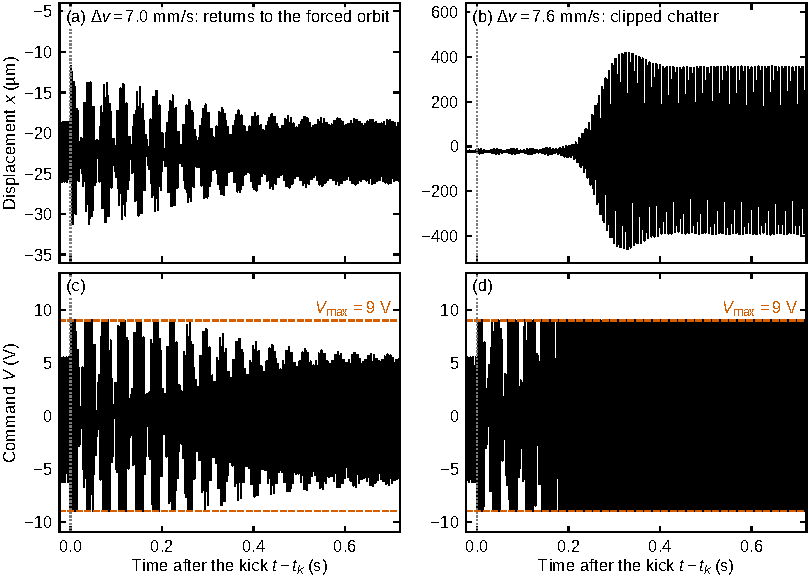
\includegraphics[width=\textwidth]{figures/fig03_two_outcomes.pdf}
  \caption{The same linearly stable cut (\SI{2500}{\rpm}, $g=\SI{1500}{\volt\second\per\metre}$, $a=0.9a_{\lim}=\SI{15.51}{\milli\metre}$, $\lvert V\rvert\le\SI{9}{\volt}$), settled by a face entry and kicked at the start of a tooth period (critical kick \SI{7.29}{\milli\metre\per\second}). (a,\,c)~$\Delta v=\SI{7.0}{\milli\metre\per\second}$: return to the forced orbit. (b,\,d)~$\Delta v=\SI{7.6}{\milli\metre\per\second}$: clipped chatter. Top: displacement $x$; bottom: command $V$ and clip $\pm V_{\max}$; dotted line: the kick.}
  \label{fig:two}
\end{figure}
% src: paper/figures/figure_numbers.json (fig03), results/c1_basin.npz

\subsection{Entry limits over 251 speeds}\label{sec:bistab-map}

With the step entry the ratio of the clipped limit to $\alim$ has a median of 0.910 and a minimum of 0.736 (\SI{2460}{\rpm}), and it is below $0.97\alim$ at 157 of 251 speeds (Fig.~\ref{fig:map}). The face entry reaches at least $0.985\alim$ at every speed. Without the clip the step-entry limit sits at the linear limit (median ratio 1.01; Supplementary Material, Sections~\ref{S-supp:bistab-map} and~\ref{S-supp:std-bistab-map}; gains up to \SI{3000}{\volt\second\per\metre}: Section~\ref{S-supp:std-bistab-gain}).
% src: results/c1_map.npz, results/c1_summary.json (map: step_clip, edge_clip, step_free); results/c1_map.npz recomputed: a_step_free/a_lim > 1.015 at 75 speeds (1.0165-1.050); a_edge_clip and a_feed_clip = 1.05 a_lim at 500, 540, 670, 720, 1000, 1080 rpm, a_step_clip at 500, 550, 670, 1000 rpm (seven speeds in all); at the other 245 speeds a_edge_clip mean 18.200 mm, a_lim mean 18.206 mm; results/feas_g1500.npz (at_bound: 157) vs results/c1_map.npz (a_step_clip < 0.97 a_lim: 157), 110 in common; verification/tdsim/check10_forced_resonance_long_runs.json

The lower edge of the unsafe band was found at 109 of the 126 speeds, at 0.21--$0.98\alim$ (median 0.46), and always above the uncontrolled limit, at no less than $1.08\alim(0)$. The edge rests on kicks of up to \SI{3}{\metre\per\second}, far beyond the validity of the model, and the bisection assumes that the band has no holes in depth; a scan of the depth at nine speeds confirms the edge at all of them but finds a hole at one.
% src: results/c1_band.npz, results/c1_summary.json (band: found 109/126, ratio 0.21/0.46/0.98, over_alim0_min 1.08); README §11.4
% src: verification/paper/protocol_band_holes.json (summary.all: speeds_complete 9, speeds_with_holes [520], speeds_with_chatter_below_edge [], total_runs 2028; grid_edge_frac next to stored_edge_frac at all nine speeds)

\begin{figure}[!tbp]
  \centering
  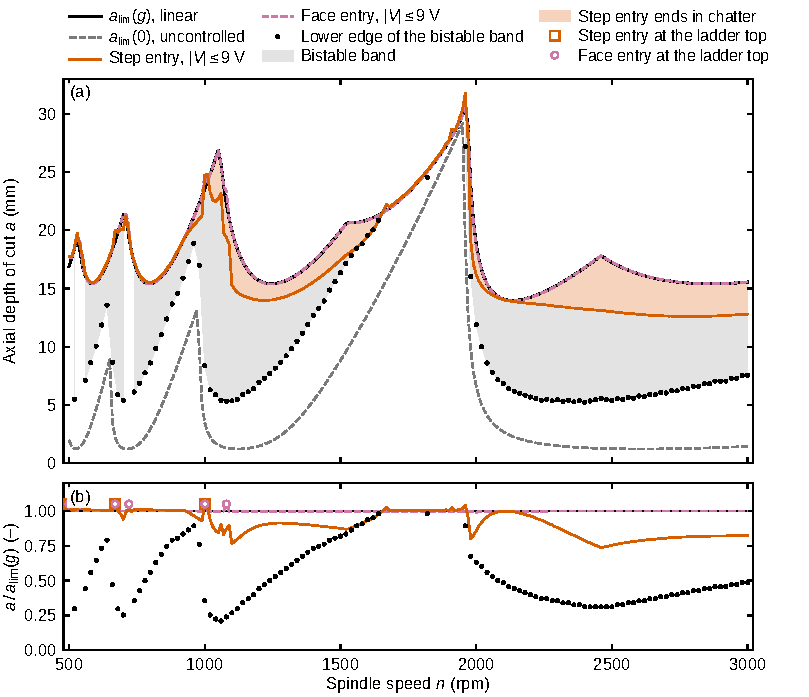
\includegraphics[width=0.86\textwidth]{figures/fig04_entry_map.pdf}
  \caption{Depth limits over 251 speeds with the gains of Section~\ref{sec:feasibility} ($\mathcal G=[0,1500]$). (a)~Linear limit $a_{\lim}(g)$, uncontrolled limit $a_{\lim}(0)$, time-domain limits with the \SI{9}{\volt} clip for the step and the face entry, and lower edge of the unsafe band (every \SI{20}{\rpm}). Shaded: the unsafe band, and the part of it in which the step entry ends in chatter. (b)~The same limits as fractions of $a_{\lim}(g)$; open markers: step-entry (squares) and face-entry (circles) limits at the top of the depth ladder, $1.05a_{\lim}$, above which they were not resolved.}
  \label{fig:map}
\end{figure}

\subsection{Basin of the forced orbit}\label{sec:bistab-basin}

Figure~\ref{fig:basin} gives the critical kick at 1090, 1420, 2500 and \SI{2870}{\rpm} with $g=1500$, at twelve depths from 0.15 to $0.98\alim$ with the clip and at four without it (Table~\ref{S-tab:basin}). With the clip the basin is finite from 0.25--$0.80\alim$ onwards and narrows towards the limit. The impulse of the kick, $m\Delta v^*$, is compared with the mean cutting impulse of one tooth period,
\begin{equation}\label{eq:impulse}
  \bar F_yT,\qquad \bar F_y=\frac{N_t\,a\,f_z}{2\pi}\Bigl(\frac{\pi}{4}K_{tc}+\frac12K_{rc}\Bigr),
\end{equation}
where $\bar F_y$ is the mean static force normal to the feed. At $0.98\alim$ the critical kick of the worst phase carries \SIrange{2.4}{10.8}{\percent} of this impulse. At this depth, changes of kick timing, observation window and number of phases alter it by at most \SI{1.1}{\percent}\phantomsection\label{sec:bistab-checks} (Supplementary Material, Section~\ref{S-supp:bistab-checks}).
% src: results/c1_basin.npz (dv, frac, vmax, tooth_impulse, mass), results/c1_summary.json (basin: first_finite_frac, impulse_098_pct, impulse_098_min_pct); src/c1_unsafe_zone.py (run_basin: tooth impulse); README §11.5
% src: verification/paper/protocol_phases.json (summary: n_phases_available 64 at all four speeds; min over 64 phases against 16 at 0.98 a_lim: rel_change_of_min -0.0108 at 1090 rpm, 0 at 1420, 2500, 2870 rpm; all.largest_drop_of_min -0.0108); verification/paper/protocol_window.json (summary: 4 points, 53 runs, n_disagreeing_runs 0, ratio 1.0 at 1090/1420/2500/2870 rpm); verification/paper/protocol_kick_timing.json (summary.all: 16 points, ratio 0.989-1, max_abs_rel_change 0.0108; per speed ratio_of_minima 1.0; reproduction_all_identical true)

\begin{figure}[!tbp]
  \centering
  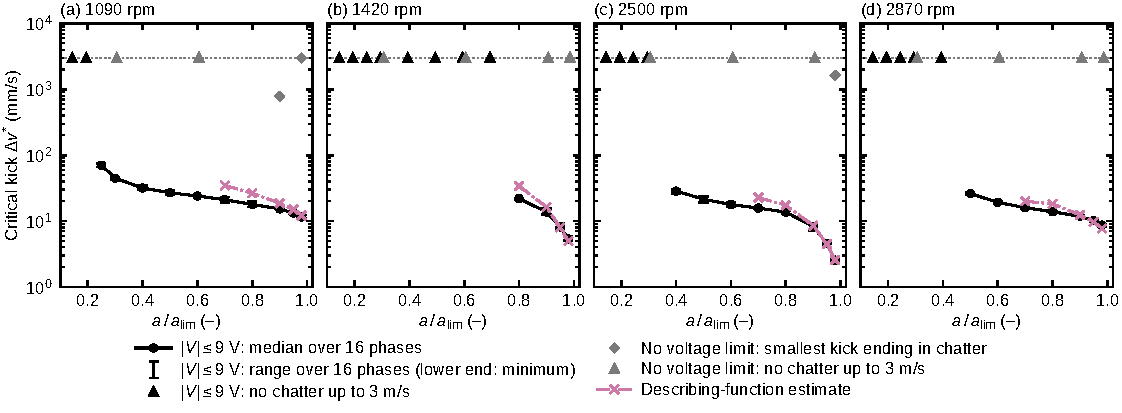
\includegraphics[width=\textwidth]{figures/fig05_basin.pdf}
  \caption{Critical kick $\Delta v^*$ against $a/a_{\lim}$ at (a)~1090, (b)~1420, (c)~2500 and (d)~\SI{2870}{\rpm} ($g=\SI{1500}{\volt\second\per\metre}$). With the \SI{9}{\volt} clip: median over 16 phases (circles) and range over the phases (bars; lower end: worst phase); black triangles: no chatter for any kick up to \SI{3}{\metre\per\second}. Without the clip: smallest kick that ends in chatter (diamonds), or none up to \SI{3}{\metre\per\second} (grey triangles). Crosses: describing-function estimate, Eq.~\eqref{eq:dfbasin}. Right axis of (d): $\Delta v^*/\omega_n$.}
  \label{fig:basin}
\end{figure}

\subsection{What lies beyond the basin}\label{sec:bistab-attr}

At the 29 points of Fig.~\ref{fig:basin} where the basin is finite, kicks at the worst phase of 2, 2.5 and 3 times the critical kick, followed for 2000 revolutions, all ended in bounded, stationary chatter with a peak-to-peak displacement of 0.08--\SI{2.0}{\milli\metre}, so that the tool leaves the cut periodically, which bounds the amplitude \citep{tlusty1981basic}. Bifurcation-type diagrams at the four speeds place this quasi-periodic chatter from within \SI{0.15}{\milli\metre} of the edge of the unsafe band up to the linear limit, coexisting with the forced orbit: over these ranges the clipped cut is bistable (Fig.~\ref{S-fig:attr}). At five of 14 further speeds where the band reaches deep cuts, a disturbance threw the model beyond the \SI{1}{\centi\metre} stop; with the stop at \SI{10}{\centi\metre}, all 21 such runs returned to the forced orbit after excursions of 12--\SI{30}{\milli\metre}, which no real cut would survive: the band map counts them as chatter, but they are not bistability.
% src: verification/paper/attractors_kick.json (summary: 29 points run, 87 runs, outcome_counts bounded_stationary 87; Q4 pp_x 0.081-1.993 mm)
% src: verification/paper/attractors_bifurcation.json/.npz (28 depths a_lim(0)-1.05 a_lim, ICs face, kick0.3, kick0.03, step, NREV 1600; states forced/chatter only, no diverged); verification/paper/attractors_summary.json (high_branch_end_minus_band_edge_mm -0.088, -0.103, -0.005, -0.150 against results/c1_band.npz, interpolated at 1090 and 2870 rpm); paper/figures/figure_numbers.json (fig_attr: bifurcation, spectra_2500_09 peak 134.6 Hz); verification/paper/attractors_chaos.json (10 cases, verdict regular, sep_final_over_pp <= 4.9e-7)
% src: verification/paper/attractors_band_spot.json (summary: 14 speeds, 78 runs, state_counts forced 34, diverged (|x| > 1 cm) 21, chatter 23; speeds_with_divergence 700, 1020, 1040, 1050, 1060); verification/paper/attractors_abort.json (abort 0.1 m: 21/21 forced, max_x 12.5-30.3 mm, back on the forced orbit after 18-59 revolutions, D1 stable)

\subsection{A describing-function prediction}\label{sec:bistab-df}

The size of the basin near the limit can be predicted with a dual-input describing function \citep{gelb1968describing}. Near the limit the deviation from the orbit is dominated by the chatter mode, and the unclipped command is $u=b(t)+A\sin\omega_ct$, with $A$ the amplitude of its chatter component and $\omega_c$ the chatter frequency. For $\omega_c$ incommensurate with $\omega_T$, the clip acts on the chatter component as the gain
\begin{equation}\label{eq:df}
  \mathcal N(A)=\lim_{\tau_a\to\infty}\frac{2}{A\tau_a}\int_0^{\tau_a}\operatorname{sat}_{V_{\max}}\bigl(b(t)+A\sin\omega_ct\bigr)\sin\omega_ct\,\mathrm dt\ \le 1,
\end{equation}
and the clipped loop thus behaves like DVF with the effective gain $\mathcal N(A)\,g$. A cut of depth $a<\alim(g)$ needs only the gain $g_e(a)$, the largest gain not above $g$ with $\alim(g_e)=a$, and chatter can be sustained once the gain of Eq.~\eqref{eq:df} falls below $g_e(a)/g$, i.e.\ above a critical amplitude $A^*(a)$. A kick $\Delta v$ excites the chatter mode with a velocity amplitude $p\,\Delta v$, where $p$ was fitted on the unclipped cut (Supplementary Material, Sections~\ref{S-supp:bistab-df} and~\ref{S-supp:std-bistab-df}). Hence
\begin{equation}\label{eq:dfbasin}
  \Delta v^*_{\mathrm{DF}}(a)=\frac{A^*(a)}{g\,p},\qquad
  \Delta v^*_{\mathrm{DF}}\;\to\;\frac{V_{\max}-b_{\max}}{g\,p}\quad\text{as }a\to a_{\lim}.
\end{equation}
% src: src/c1_unsafe_zone.py (df_gain: 128 phases, b on 128 samples per tooth period; critical_amplitude; effective_gain_needed; _mode_factor: kick of 1 mm/s at phase 0, high-pass 40 Hz, fit of the slowest decaying mode)

Where $p$ could be fitted, from 0.7--$0.8\alim$ upwards, the simulated critical kick (median over the phases) is 0.61--1.13 times this estimate, and 0.88--1.13 times at 0.95 and $0.98\alim$ (Fig.~\ref{fig:basin}). Equation~\eqref{eq:dfbasin} predicts, without proving it, that the basin does not close at the limit but tends to a finite size set by the residual authority. The estimate rests on the filtering hypothesis and on the factor $p$, fitted at one kick phase and valid only near the limit.
% src: results/c1_df.npz (A_dual at a = a_lim = V_max - b_max), results/c1_basin.npz (p_mode finite at frac >= 0.7, at 1420 rpm >= 0.8), results/c1_summary.json (td_over_df 0.61-1.13); ratios at 0.95/0.98 recomputed with the c1_summary formula: 0.88-1.13; README §11.5
